% Options for packages loaded elsewhere
\PassOptionsToPackage{unicode}{hyperref}
\PassOptionsToPackage{hyphens}{url}
\PassOptionsToPackage{dvipsnames,svgnames,x11names}{xcolor}
%
\documentclass[
  ignorenonframetext,
]{beamer}
\usepackage{pgfpages}
\setbeamertemplate{caption}[numbered]
\setbeamertemplate{caption label separator}{: }
\setbeamercolor{caption name}{fg=normal text.fg}
\beamertemplatenavigationsymbolsempty
% Prevent slide breaks in the middle of a paragraph
\widowpenalties 1 10000
\raggedbottom
\setbeamertemplate{part page}{
  \centering
  \begin{beamercolorbox}[sep=16pt,center]{part title}
    \usebeamerfont{part title}\insertpart\par
  \end{beamercolorbox}
}
\setbeamertemplate{section page}{
  \centering
  \begin{beamercolorbox}[sep=12pt,center]{part title}
    \usebeamerfont{section title}\insertsection\par
  \end{beamercolorbox}
}
\setbeamertemplate{subsection page}{
  \centering
  \begin{beamercolorbox}[sep=8pt,center]{part title}
    \usebeamerfont{subsection title}\insertsubsection\par
  \end{beamercolorbox}
}
\AtBeginPart{
  \frame{\partpage}
}
\AtBeginSection{
  \ifbibliography
  \else
    \frame{\sectionpage}
  \fi
}
\AtBeginSubsection{
  \frame{\subsectionpage}
}
\usepackage{amsmath,amssymb}
\usepackage{lmodern}
\usepackage{iftex}
\ifPDFTeX
  \usepackage[T1]{fontenc}
  \usepackage[utf8]{inputenc}
  \usepackage{textcomp} % provide euro and other symbols
\else % if luatex or xetex
  \usepackage{unicode-math}
  \defaultfontfeatures{Scale=MatchLowercase}
  \defaultfontfeatures[\rmfamily]{Ligatures=TeX,Scale=1}
\fi
% Use upquote if available, for straight quotes in verbatim environments
\IfFileExists{upquote.sty}{\usepackage{upquote}}{}
\IfFileExists{microtype.sty}{% use microtype if available
  \usepackage[]{microtype}
  \UseMicrotypeSet[protrusion]{basicmath} % disable protrusion for tt fonts
}{}
\makeatletter
\@ifundefined{KOMAClassName}{% if non-KOMA class
  \IfFileExists{parskip.sty}{%
    \usepackage{parskip}
  }{% else
    \setlength{\parindent}{0pt}
    \setlength{\parskip}{6pt plus 2pt minus 1pt}}
}{% if KOMA class
  \KOMAoptions{parskip=half}}
\makeatother
\usepackage{xcolor}
\newif\ifbibliography
\usepackage{color}
\usepackage{fancyvrb}
\newcommand{\VerbBar}{|}
\newcommand{\VERB}{\Verb[commandchars=\\\{\}]}
\DefineVerbatimEnvironment{Highlighting}{Verbatim}{commandchars=\\\{\}}
% Add ',fontsize=\small' for more characters per line
\usepackage{framed}
\definecolor{shadecolor}{RGB}{248,248,248}
\newenvironment{Shaded}{\begin{snugshade}}{\end{snugshade}}
\newcommand{\AlertTok}[1]{\textcolor[rgb]{0.94,0.16,0.16}{#1}}
\newcommand{\AnnotationTok}[1]{\textcolor[rgb]{0.56,0.35,0.01}{\textbf{\textit{#1}}}}
\newcommand{\AttributeTok}[1]{\textcolor[rgb]{0.77,0.63,0.00}{#1}}
\newcommand{\BaseNTok}[1]{\textcolor[rgb]{0.00,0.00,0.81}{#1}}
\newcommand{\BuiltInTok}[1]{#1}
\newcommand{\CharTok}[1]{\textcolor[rgb]{0.31,0.60,0.02}{#1}}
\newcommand{\CommentTok}[1]{\textcolor[rgb]{0.56,0.35,0.01}{\textit{#1}}}
\newcommand{\CommentVarTok}[1]{\textcolor[rgb]{0.56,0.35,0.01}{\textbf{\textit{#1}}}}
\newcommand{\ConstantTok}[1]{\textcolor[rgb]{0.00,0.00,0.00}{#1}}
\newcommand{\ControlFlowTok}[1]{\textcolor[rgb]{0.13,0.29,0.53}{\textbf{#1}}}
\newcommand{\DataTypeTok}[1]{\textcolor[rgb]{0.13,0.29,0.53}{#1}}
\newcommand{\DecValTok}[1]{\textcolor[rgb]{0.00,0.00,0.81}{#1}}
\newcommand{\DocumentationTok}[1]{\textcolor[rgb]{0.56,0.35,0.01}{\textbf{\textit{#1}}}}
\newcommand{\ErrorTok}[1]{\textcolor[rgb]{0.64,0.00,0.00}{\textbf{#1}}}
\newcommand{\ExtensionTok}[1]{#1}
\newcommand{\FloatTok}[1]{\textcolor[rgb]{0.00,0.00,0.81}{#1}}
\newcommand{\FunctionTok}[1]{\textcolor[rgb]{0.00,0.00,0.00}{#1}}
\newcommand{\ImportTok}[1]{#1}
\newcommand{\InformationTok}[1]{\textcolor[rgb]{0.56,0.35,0.01}{\textbf{\textit{#1}}}}
\newcommand{\KeywordTok}[1]{\textcolor[rgb]{0.13,0.29,0.53}{\textbf{#1}}}
\newcommand{\NormalTok}[1]{#1}
\newcommand{\OperatorTok}[1]{\textcolor[rgb]{0.81,0.36,0.00}{\textbf{#1}}}
\newcommand{\OtherTok}[1]{\textcolor[rgb]{0.56,0.35,0.01}{#1}}
\newcommand{\PreprocessorTok}[1]{\textcolor[rgb]{0.56,0.35,0.01}{\textit{#1}}}
\newcommand{\RegionMarkerTok}[1]{#1}
\newcommand{\SpecialCharTok}[1]{\textcolor[rgb]{0.00,0.00,0.00}{#1}}
\newcommand{\SpecialStringTok}[1]{\textcolor[rgb]{0.31,0.60,0.02}{#1}}
\newcommand{\StringTok}[1]{\textcolor[rgb]{0.31,0.60,0.02}{#1}}
\newcommand{\VariableTok}[1]{\textcolor[rgb]{0.00,0.00,0.00}{#1}}
\newcommand{\VerbatimStringTok}[1]{\textcolor[rgb]{0.31,0.60,0.02}{#1}}
\newcommand{\WarningTok}[1]{\textcolor[rgb]{0.56,0.35,0.01}{\textbf{\textit{#1}}}}
\usepackage{graphicx}
\makeatletter
\def\maxwidth{\ifdim\Gin@nat@width>\linewidth\linewidth\else\Gin@nat@width\fi}
\def\maxheight{\ifdim\Gin@nat@height>\textheight\textheight\else\Gin@nat@height\fi}
\makeatother
% Scale images if necessary, so that they will not overflow the page
% margins by default, and it is still possible to overwrite the defaults
% using explicit options in \includegraphics[width, height, ...]{}
\setkeys{Gin}{width=\maxwidth,height=\maxheight,keepaspectratio}
% Set default figure placement to htbp
\makeatletter
\def\fps@figure{htbp}
\makeatother
\setlength{\emergencystretch}{3em} % prevent overfull lines
\providecommand{\tightlist}{%
  \setlength{\itemsep}{0pt}\setlength{\parskip}{0pt}}
\setcounter{secnumdepth}{-\maxdimen} % remove section numbering
\usepackage{graphicx}
\usepackage{bm}
\definecolor{foreground}{RGB}{255,255,255}
\definecolor{background}{RGB}{34,28,54}
\definecolor{title}{RGB}{105,165,255}
\definecolor{gray}{RGB}{175,175,175}
\definecolor{lightgray}{RGB}{225,225,225}
\definecolor{subtitle}{RGB}{232,234,255}
\definecolor{hilight}{RGB}{112,224,255}
\definecolor{vhilight}{RGB}{255,111,207}
\setbeamertemplate{footline}[page number]
\ifLuaTeX
  \usepackage{selnolig}  % disable illegal ligatures
\fi
\IfFileExists{bookmark.sty}{\usepackage{bookmark}}{\usepackage{hyperref}}
\IfFileExists{xurl.sty}{\usepackage{xurl}}{} % add URL line breaks if available
\urlstyle{same} % disable monospaced font for URLs
\hypersetup{
  pdftitle={STAT 528 - Advanced Regression Analysis II},
  pdfauthor={Linear Mixed Models},
  colorlinks=true,
  linkcolor={Maroon},
  filecolor={Maroon},
  citecolor={Blue},
  urlcolor={blue},
  pdfcreator={LaTeX via pandoc}}

\title{STAT 528 - Advanced Regression Analysis II}
\author{Linear Mixed Models}
\date{}
\institute{Daniel J. Eck\\
Department of Statistics\\
University of Illinois}

\begin{document}
\frame{\titlepage}

\begin{frame}{Learning Objectives Today}
\protect\hypertarget{learning-objectives-today}{}
\begin{itemize}
\tightlist
\item
  Linear Mixed Models examples
\end{itemize}
\end{frame}

\begin{frame}{Example: pulp data set}
\protect\hypertarget{example-pulp-data-set}{}
We illustrate the fitting methods using some data from an experiment
which tests how the paper brightness is influenced by the shift operator
on duty.

The pulp data frame has 20 rows and 2 columns. Data comes from an
experiment to test the paper brightness depending on a shift operator.
The variables are:

\begin{itemize}
\tightlist
\item
  \textbf{bright}: Brightness of the pulp as measured by a reflectance
  meter
\item
  \textbf{operator}: Shift operator a-d
\end{itemize}
\end{frame}

\begin{frame}[fragile]{}
\protect\hypertarget{section}{}
We start with a fixed effects one-way ANOVA.

\vspace{12pt}
\tiny

\begin{Shaded}
\begin{Highlighting}[]
\FunctionTok{library}\NormalTok{(ggplot2)}
\FunctionTok{library}\NormalTok{(faraway)}
\FunctionTok{data}\NormalTok{(pulp)}
\DocumentationTok{\#\# note that we are changing the contrasts to sum contrasts}
\NormalTok{op }\OtherTok{\textless{}{-}} \FunctionTok{options}\NormalTok{(}\AttributeTok{contrasts =} \FunctionTok{c}\NormalTok{(}\StringTok{"contr.sum"}\NormalTok{, }\StringTok{"contr.poly"}\NormalTok{))}
\DocumentationTok{\#\# aov is another wrapper for lm; results more appropriate for ANOVA models}
\NormalTok{lmod }\OtherTok{\textless{}{-}} \FunctionTok{aov}\NormalTok{(bright }\SpecialCharTok{\textasciitilde{}}\NormalTok{ operator, pulp)}
\FunctionTok{summary}\NormalTok{(lmod)}
\end{Highlighting}
\end{Shaded}

\begin{verbatim}
##             Df Sum Sq Mean Sq F value Pr(>F)  
## operator     3   1.34  0.4467   4.204 0.0226 *
## Residuals   16   1.70  0.1062                 
## ---
## Signif. codes:  0 '***' 0.001 '**' 0.01 '*' 0.05 '.' 0.1 ' ' 1
\end{verbatim}

\begin{Shaded}
\begin{Highlighting}[]
\FunctionTok{coef}\NormalTok{(lmod)}
\end{Highlighting}
\end{Shaded}

\begin{verbatim}
## (Intercept)   operator1   operator2   operator3 
##       60.40       -0.16       -0.34        0.22
\end{verbatim}
\end{frame}

\begin{frame}[fragile]{}
\protect\hypertarget{section-1}{}
We see that the p-value for the operator effect is roughly 0.023. We
have \(\hat{\sigma}^2 = .106\) and the overall mean is 60.40.

For sum contrasts, we have that \(\sum_i\alpha_i = 0\), so we can
calculate the effect for the fourth operator as 0.16 + 0.34 - 0.22 =
0.28.

Turing to the random effects model, we can calculate the variance of the
operator effects \(\hat{\sigma}^2_{\alpha}\) using the formula above as

\vspace{12pt}

\begin{Shaded}
\begin{Highlighting}[]
\DocumentationTok{\#\# (MSA {-} MSE) / n }
\NormalTok{(}\FloatTok{0.4467} \SpecialCharTok{{-}} \FloatTok{0.1062}\NormalTok{)}\SpecialCharTok{/}\DecValTok{5}
\end{Highlighting}
\end{Shaded}

\begin{verbatim}
## [1] 0.0681
\end{verbatim}
\end{frame}

\begin{frame}[fragile]{}
\protect\hypertarget{section-2}{}
We now demonstrate the MLE approach using REML. We will use the
\texttt{lme4} package to accomplish this task.

\vspace{12pt}
\tiny

\begin{Shaded}
\begin{Highlighting}[]
\FunctionTok{library}\NormalTok{(lme4)}
\NormalTok{mmod }\OtherTok{\textless{}{-}} \FunctionTok{lmer}\NormalTok{(bright }\SpecialCharTok{\textasciitilde{}} \DecValTok{1} \SpecialCharTok{+}\NormalTok{ (}\DecValTok{1}\SpecialCharTok{|}\NormalTok{operator), pulp)}
\FunctionTok{summary}\NormalTok{(mmod)}
\end{Highlighting}
\end{Shaded}

\begin{verbatim}
## Linear mixed model fit by REML ['lmerMod']
## Formula: bright ~ 1 + (1 | operator)
##    Data: pulp
## 
## REML criterion at convergence: 18.6
## 
## Scaled residuals: 
##     Min      1Q  Median      3Q     Max 
## -1.4666 -0.7595 -0.1244  0.6281  1.6012 
## 
## Random effects:
##  Groups   Name        Variance Std.Dev.
##  operator (Intercept) 0.06808  0.2609  
##  Residual             0.10625  0.3260  
## Number of obs: 20, groups:  operator, 4
## 
## Fixed effects:
##             Estimate Std. Error t value
## (Intercept)  60.4000     0.1494   404.2
\end{verbatim}

\vspace{12pt}
\normalsize

We see that this method gives identical estimates to the ANOVA results
above. For unbalanced designs, the REML and ANOVA estimators are not
necessarily identical.
\end{frame}

\begin{frame}{}
\protect\hypertarget{section-3}{}
The model fitted has both fixed and random effects components.

The fixed effect here is just the intercept represented by the first
\texttt{1} in the model formula.

The random effect is represented by the \texttt{(1|operator)} indicating
that the data is grouped by the \texttt{operator} variable, and the
\texttt{1} indicates that the random effect is constant within each
group.
\end{frame}

\begin{frame}{LRT}
\protect\hypertarget{lrt}{}
In this example the only fixed effect is the mean and there is not much
interest in testing that.

For models of the same class, we could use built in software to perform
a statistical test. Here we have to do the testing manually
\end{frame}

\begin{frame}[fragile]{}
\protect\hypertarget{section-4}{}
\vspace{12pt}
\small

\begin{Shaded}
\begin{Highlighting}[]
\DocumentationTok{\#\# null model fit}
\NormalTok{nullmod }\OtherTok{\textless{}{-}} \FunctionTok{lm}\NormalTok{(bright }\SpecialCharTok{\textasciitilde{}} \DecValTok{1}\NormalTok{, pulp) }

\DocumentationTok{\#\# alternative model fit}
\NormalTok{smod }\OtherTok{\textless{}{-}} \FunctionTok{lmer}\NormalTok{(bright }\SpecialCharTok{\textasciitilde{}} \DecValTok{1} \SpecialCharTok{+}\NormalTok{ (}\DecValTok{1}\SpecialCharTok{|}\NormalTok{operator), pulp, }\AttributeTok{REML =} \ConstantTok{FALSE}\NormalTok{)}

\DocumentationTok{\#\# LRT}
\FunctionTok{as.numeric}\NormalTok{(}\DecValTok{2}\SpecialCharTok{*}\NormalTok{(}\FunctionTok{logLik}\NormalTok{(smod) }\SpecialCharTok{{-}} \FunctionTok{logLik}\NormalTok{(nullmod)))}
\end{Highlighting}
\end{Shaded}

\begin{verbatim}
## [1] 2.568371
\end{verbatim}

\begin{Shaded}
\begin{Highlighting}[]
\FunctionTok{pchisq}\NormalTok{(}\FloatTok{2.568371}\NormalTok{, }\AttributeTok{df =} \DecValTok{1}\NormalTok{, }\AttributeTok{lower =} \ConstantTok{FALSE}\NormalTok{)}
\end{Highlighting}
\end{Shaded}

\begin{verbatim}
## [1] 0.1090199
\end{verbatim}
\end{frame}

\begin{frame}{}
\protect\hypertarget{section-5}{}
The \(p\)-value for this test is well above a nominal 5\% significance
level (assuming that testing is desired at this level). The use of the
\(\chi^2\) test with its noted shortcomings allows for some doubt in
this finding.

We will now try the parametric bootstrap procedure to obtain a more
accurate \(p\)-value. We need to estimate the probability, given the
null hypothesis is true, of observation an LRT of 2.568371 or greater.

We have that \[
  y \overset{H_0}{\sim} N(\mu,\sigma^2).
\]
\end{frame}

\begin{frame}{}
\protect\hypertarget{section-6}{}
A simulation approach would generate data under this model, fit the null
and alternative models and then compute the LRT.

The process would be repeated a large number of times and the proportion
of estimated LRTs exceeding the the observed LRT value of 2.568371 would
be used to estimate the \(p\)-value. In practice we do not know the true
values of \(\mu\) and \(\sigma\), but we can use plug-in.

Let's try it out. Fix the bootstrap sample size to be \(B = 1000\) and
then continue with the parametric bootstrap procedure.
\end{frame}

\begin{frame}[fragile]{parametric bootstrap}
\protect\hypertarget{parametric-bootstrap}{}
\tiny

\begin{Shaded}
\begin{Highlighting}[]
\FunctionTok{set.seed}\NormalTok{(}\DecValTok{13}\NormalTok{)}
\NormalTok{B }\OtherTok{\textless{}{-}} \DecValTok{1000}
\NormalTok{lrtstat }\OtherTok{\textless{}{-}} \FunctionTok{numeric}\NormalTok{(B)}
\FunctionTok{system.time}\NormalTok{(}\ControlFlowTok{for}\NormalTok{(b }\ControlFlowTok{in} \DecValTok{1}\SpecialCharTok{:}\NormalTok{B)\{}
\NormalTok{  y }\OtherTok{\textless{}{-}} \FunctionTok{unlist}\NormalTok{(}\FunctionTok{simulate}\NormalTok{(nullmod))}
\NormalTok{  bnull }\OtherTok{\textless{}{-}} \FunctionTok{lm}\NormalTok{(y }\SpecialCharTok{\textasciitilde{}} \DecValTok{1}\NormalTok{)}
\NormalTok{  balt }\OtherTok{\textless{}{-}} \FunctionTok{lmer}\NormalTok{(y }\SpecialCharTok{\textasciitilde{}} \DecValTok{1} \SpecialCharTok{+}\NormalTok{ (}\DecValTok{1}\SpecialCharTok{|}\NormalTok{operator), pulp, }\AttributeTok{REML =} \ConstantTok{FALSE}\NormalTok{)}
\NormalTok{  lrtstat[b] }\OtherTok{\textless{}{-}} \FunctionTok{as.numeric}\NormalTok{(}\DecValTok{2}\SpecialCharTok{*}\NormalTok{(}\FunctionTok{logLik}\NormalTok{(balt) }\SpecialCharTok{{-}} \FunctionTok{logLik}\NormalTok{(bnull)))}
\NormalTok{\})}
\end{Highlighting}
\end{Shaded}

\begin{verbatim}
##    user  system elapsed 
##   5.667   0.046   5.714
\end{verbatim}

\vspace{12pt}
\normalsize

We may examine the distribution of the bootstrapped LRTs. We first
compute the proportion that are close to zero

\vspace{12pt}
\tiny

\begin{Shaded}
\begin{Highlighting}[]
\FunctionTok{mean}\NormalTok{(lrtstat }\SpecialCharTok{\textless{}} \FloatTok{1e{-}5}\NormalTok{)}
\end{Highlighting}
\end{Shaded}

\begin{verbatim}
## [1] 0.69
\end{verbatim}
\end{frame}

\begin{frame}[fragile]{}
\protect\hypertarget{section-7}{}
The LRT clearly does not have a \(\chi^2\) distribution. See Section 8.2
in Faraway for discussion on this. An interesting refinement can be seen
\href{https://www.sciencedirect.com/science/article/pii/S0167947307004306?casa_token=z-BkV1gXcLQAAAAA:FbUGOMy6WR2WFBfIZ2e1OfpJBpzhhQd4zc3OFtNjUGiaCdlXKa4yQOwbw3xcgPXQ-JaZMbUuLQ}{here}.

The parametric bootstrap may be the simplest approach, and the method we
have used above is transparent and could be computed much more
efficiently if needed. With all of this in mind the estimated
\(p\)-value is

\vspace{12pt}
\tiny

\begin{Shaded}
\begin{Highlighting}[]
\DocumentationTok{\#\# p{-}value}
\NormalTok{pval }\OtherTok{\textless{}{-}} \FunctionTok{mean}\NormalTok{(lrtstat }\SpecialCharTok{\textgreater{}} \FloatTok{2.568371}\NormalTok{)}
\NormalTok{pval}
\end{Highlighting}
\end{Shaded}

\begin{verbatim}
## [1] 0.026
\end{verbatim}

\begin{Shaded}
\begin{Highlighting}[]
\DocumentationTok{\#\# simple standard error of the above}
\FunctionTok{sqrt}\NormalTok{(pval}\SpecialCharTok{*}\NormalTok{(}\DecValTok{1}\SpecialCharTok{{-}}\NormalTok{pval)}\SpecialCharTok{/}\NormalTok{B)}
\end{Highlighting}
\end{Shaded}

\begin{verbatim}
## [1] 0.005032296
\end{verbatim}

\vspace{12pt}
\normalsize

We can be fairly sure that the estimated \(p\)-value is under a 0.05
nominal level. If in doubt, do some more replications to make sure; this
only costs computer time. As it happens, this \(p\)-value is close to
the fixed effects \(p\)-value.
\end{frame}

\begin{frame}{Predicting random effects}
\protect\hypertarget{predicting-random-effects}{}
Approach this problem from a Bayesian perspective with a prior density
for the \(\alpha\)s such that \(E(\alpha_i) = 0\) is just the prior
mean.

Let \(f\) represent a density function, then the posterior density for
\(\alpha\) is given by \[
  f(\alpha_i|Y) \propto f(Y|\alpha_i)f(\alpha_i)
\] we can then find the posterior mean, denoted as \(\hat{\alpha}\) as
\[
  E(\alpha_i|Y) = \int \alpha_i f(\alpha_i|Y) d\alpha_i.
\] For the general case, this works out to be \[
  \hat\alpha = DZ^TV^{-1}(Y - X\beta).
\]
\end{frame}

\begin{frame}[fragile]{}
\protect\hypertarget{section-8}{}
We will take an empirical Bayesian point of view and substitute the MLEs
into \(D\), \(V\), and \(\beta\) to obtain predicted random effects.

These are be computed as

\vspace{12pt}
\tiny

\begin{Shaded}
\begin{Highlighting}[]
\FunctionTok{ranef}\NormalTok{(mmod)}\SpecialCharTok{$}\NormalTok{operator}
\end{Highlighting}
\end{Shaded}

\begin{verbatim}
##   (Intercept)
## a  -0.1219403
## b  -0.2591231
## c   0.1676679
## d   0.2133955
\end{verbatim}

\vspace{12pt}
\normalsize

The predicted random effects are related to the fixed effects. We can
show these for all operators

\vspace{12pt}
\tiny

\begin{Shaded}
\begin{Highlighting}[]
\NormalTok{(cc }\OtherTok{\textless{}{-}} \FunctionTok{model.tables}\NormalTok{(lmod))}
\end{Highlighting}
\end{Shaded}

\begin{verbatim}
## Tables of effects
## 
##  operator 
## operator
##     a     b     c     d 
## -0.16 -0.34  0.22  0.28
\end{verbatim}
\end{frame}

\begin{frame}[fragile]{}
\protect\hypertarget{section-9}{}
Look what happens when we compute the ratio of fixed effects to the
random effects

\vspace{12pt}

\begin{Shaded}
\begin{Highlighting}[]
\DocumentationTok{\#\# estimated fixed effects divided by }
\DocumentationTok{\#\# predicted random effects}
\NormalTok{cc[[}\DecValTok{1}\NormalTok{]]}\SpecialCharTok{$}\NormalTok{operator }\SpecialCharTok{/} \FunctionTok{ranef}\NormalTok{(mmod)}\SpecialCharTok{$}\NormalTok{operator}
\end{Highlighting}
\end{Shaded}

\begin{verbatim}
##   (Intercept)
## a    1.312117
## b    1.312117
## c    1.312117
## d    1.312117
\end{verbatim}

\vspace{12pt}

We see that the predicted random effects are exactly in proportion to
the fixed effects. Typically, the predicted random effects are smaller
and could be viewed as a type of \textbf{shrinkage estimate}.
\end{frame}

\begin{frame}[fragile]{}
\protect\hypertarget{section-10}{}
95\% confidence intervals for random effects:

\vspace{12pt}
\tiny

\begin{verbatim}
## $operator
\end{verbatim}

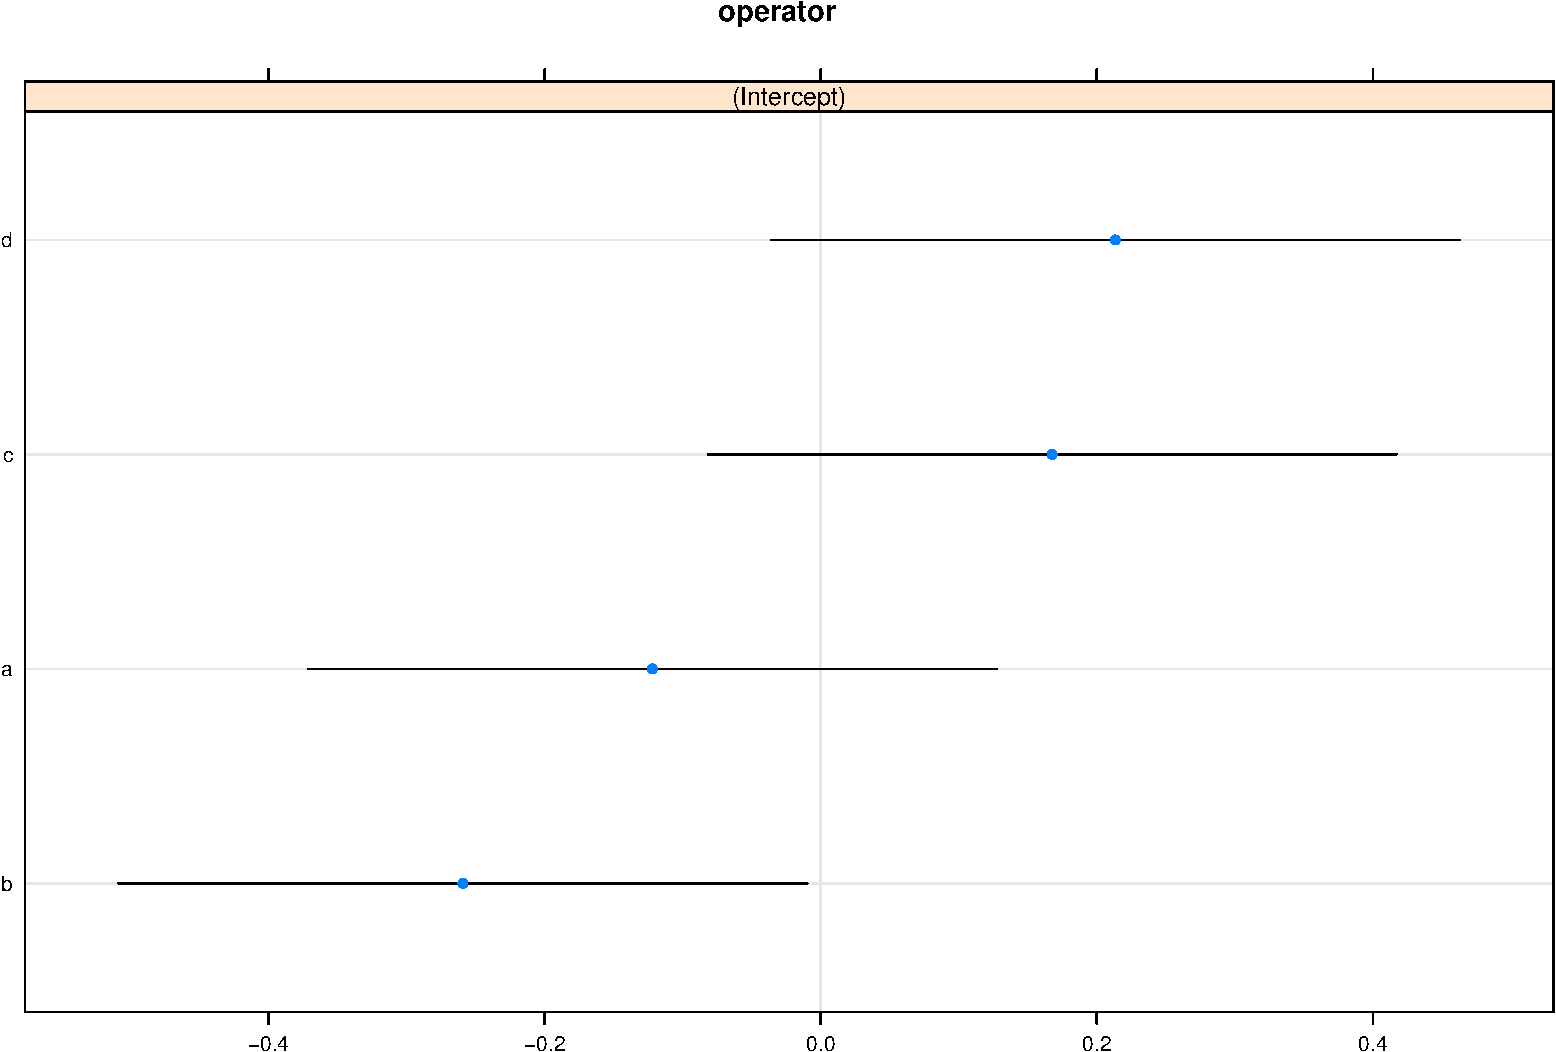
\includegraphics{week11p1_files/figure-beamer/95CI-1.pdf}
\end{frame}

\begin{frame}[fragile]{}
\protect\hypertarget{section-11}{}
Suppose we wish to predict a new value. If the prediction is to be made
for a new operator or unknown operator, the best we can do is give
\(\hat\mu = 60.4\).

If we know the operator, then we can combine this with our fixed effects
to give the best linear unbiased predictors (BLUPs) as follows

\vspace{12pt}

\begin{Shaded}
\begin{Highlighting}[]
\FunctionTok{fixef}\NormalTok{(mmod) }\SpecialCharTok{+} \FunctionTok{ranef}\NormalTok{(mmod)}\SpecialCharTok{$}\NormalTok{operator}
\end{Highlighting}
\end{Shaded}

\begin{verbatim}
##   (Intercept)
## a    60.27806
## b    60.14088
## c    60.56767
## d    60.61340
\end{verbatim}
\end{frame}

\begin{frame}{}
\protect\hypertarget{section-12}{}
We present a parametric bootstrap method for computing standard errors
of the predicted random effects.

As in previous bootstrap, the first step is to simulate from the fitted
model. We refit the model with the simulated response and generate a
predicted value.

But there are two additional sources of variation. We have variation due
to the new operator and also due to a new observation from that
operator.

For this reason, we add normal sample values with standard deviations
equal to those estimated earlier. If you really want a confidence
interval for the mean prediction, you should not add these extra error
terms.
\end{frame}

\begin{frame}[fragile]{}
\protect\hypertarget{section-13}{}
We repeat this 1000 times and take the appropriate quantiles to get a
95\% interval. We start with the unknown operator case:

\vspace{12pt}
\tiny

\begin{Shaded}
\begin{Highlighting}[]
\NormalTok{group.sd }\OtherTok{\textless{}{-}} \FunctionTok{as.data.frame}\NormalTok{(}\FunctionTok{VarCorr}\NormalTok{(mmod))}\SpecialCharTok{$}\NormalTok{sdcor[}\DecValTok{1}\NormalTok{]}
\NormalTok{resid.sd }\OtherTok{\textless{}{-}} \FunctionTok{as.data.frame}\NormalTok{(}\FunctionTok{VarCorr}\NormalTok{(mmod))}\SpecialCharTok{$}\NormalTok{sdcor[}\DecValTok{2}\NormalTok{]}
\NormalTok{B }\OtherTok{\textless{}{-}} \DecValTok{1000}
\NormalTok{pv }\OtherTok{\textless{}{-}} \FunctionTok{numeric}\NormalTok{(B)}
\FunctionTok{system.time}\NormalTok{(}\ControlFlowTok{for}\NormalTok{(i }\ControlFlowTok{in} \DecValTok{1}\SpecialCharTok{:}\NormalTok{B)\{}
\NormalTok{  y }\OtherTok{\textless{}{-}} \FunctionTok{unlist}\NormalTok{(}\FunctionTok{simulate}\NormalTok{(mmod, }\AttributeTok{use.u =} \ConstantTok{TRUE}\NormalTok{))}
\NormalTok{  bmod }\OtherTok{\textless{}{-}} \FunctionTok{suppressWarnings}\NormalTok{(}\FunctionTok{refit}\NormalTok{(mmod, y))}
\NormalTok{  pv[i] }\OtherTok{\textless{}{-}} \FunctionTok{predict}\NormalTok{(bmod, }\AttributeTok{re.form=}\SpecialCharTok{\textasciitilde{}}\DecValTok{0}\NormalTok{)[}\DecValTok{1}\NormalTok{] }\SpecialCharTok{+} \FunctionTok{rnorm}\NormalTok{(}\AttributeTok{n=}\DecValTok{1}\NormalTok{,}\AttributeTok{sd=}\NormalTok{group.sd) }\SpecialCharTok{+} 
    \FunctionTok{rnorm}\NormalTok{(}\AttributeTok{n=}\DecValTok{1}\NormalTok{,}\AttributeTok{sd=}\NormalTok{resid.sd)}
\NormalTok{\})}
\end{Highlighting}
\end{Shaded}

\begin{verbatim}
##    user  system elapsed 
##   6.683   0.051   6.735
\end{verbatim}

\begin{Shaded}
\begin{Highlighting}[]
\FunctionTok{quantile}\NormalTok{(pv, }\FunctionTok{c}\NormalTok{(}\FloatTok{0.025}\NormalTok{, }\FloatTok{0.975}\NormalTok{))}
\end{Highlighting}
\end{Shaded}

\begin{verbatim}
##     2.5%    97.5% 
## 59.62780 61.24264
\end{verbatim}
\end{frame}

\begin{frame}[fragile]{}
\protect\hypertarget{section-14}{}
Some modification is necessary if we know the operator we are making the
prediction interval for.

We use the option \texttt{use.u=TRUE} in the simulate function
indicating that we should simulate new values conditional on the
estimated random effects.

We need to do this because otherwise we would simulate an entirely new
`a' effect in each replication. Instead, we want to preserve the
originally generated `a' effect.

\vspace{12pt}
\tiny

\begin{Shaded}
\begin{Highlighting}[]
\FunctionTok{system.time}\NormalTok{(}\ControlFlowTok{for}\NormalTok{(i }\ControlFlowTok{in} \DecValTok{1}\SpecialCharTok{:}\NormalTok{B)\{}
\NormalTok{ y }\OtherTok{\textless{}{-}} \FunctionTok{unlist}\NormalTok{(}\FunctionTok{simulate}\NormalTok{(mmod, }\AttributeTok{use.u=}\ConstantTok{TRUE}\NormalTok{))}
\NormalTok{  bmod }\OtherTok{\textless{}{-}} \FunctionTok{suppressWarnings}\NormalTok{(}\FunctionTok{refit}\NormalTok{(mmod, y))}
\NormalTok{  pv[i] }\OtherTok{\textless{}{-}} \FunctionTok{predict}\NormalTok{(bmod, }\AttributeTok{newdata=}\FunctionTok{data.frame}\NormalTok{(}\AttributeTok{operator=}\StringTok{"a"}\NormalTok{)) }\SpecialCharTok{+} 
    \FunctionTok{rnorm}\NormalTok{(}\AttributeTok{n=}\DecValTok{1}\NormalTok{,}\AttributeTok{sd=}\NormalTok{resid.sd)}
\NormalTok{\})}
\end{Highlighting}
\end{Shaded}

\begin{verbatim}
##    user  system elapsed 
##   9.239   0.052   9.293
\end{verbatim}

\begin{Shaded}
\begin{Highlighting}[]
\FunctionTok{quantile}\NormalTok{(pv, }\FunctionTok{c}\NormalTok{(}\FloatTok{0.025}\NormalTok{, }\FloatTok{0.975}\NormalTok{))}
\end{Highlighting}
\end{Shaded}

\begin{verbatim}
##     2.5%    97.5% 
## 59.60897 60.97931
\end{verbatim}
\end{frame}

\begin{frame}[fragile]{Soybean Analysis (see notes)}
\protect\hypertarget{soybean-analysis-see-notes}{}
The researchers are interested in determining which genotypes are
associated with a different expression of apparent quantum efficiency
(AqE) from the RC reference genotype.

AqE is a part of the photosynthetic process in plants where improvements
in AqE allow for improvements in yield.

This data consists of multiple measurements on the same day with only a
few days of data collection.

\vspace{12pt}
\tiny

\begin{Shaded}
\begin{Highlighting}[]
\NormalTok{dat }\OtherTok{\textless{}{-}} \FunctionTok{read.csv}\NormalTok{(}\StringTok{"soybean.csv"}\NormalTok{)}
\NormalTok{dat}\SpecialCharTok{$}\NormalTok{ID }\OtherTok{\textless{}{-}} \FunctionTok{as.factor}\NormalTok{(dat}\SpecialCharTok{$}\NormalTok{ID)}
\FunctionTok{head}\NormalTok{(dat)}
\end{Highlighting}
\end{Shaded}

\begin{verbatim}
##      ID plot_number disk       AqE   Precip Precip_7day      days
## 1 NAM10         123   30 0.8237071 2.544962   0.5964009 -1.369516
## 2 NAM10          70   68 1.9022350 2.544962   0.5964009 -1.369516
## 3 NAM10         136   21 0.9653680 2.544962   0.5964009 -1.369516
## 4 NAM10         136   15 0.5140451 2.544962   0.5964009 -1.369516
## 5 NAM10          70   59 1.0306178 2.544962   0.5964009 -1.369516
## 6 NAM10          70   52 1.1022001 2.544962   0.5964009 -1.369516
\end{verbatim}
\end{frame}

\begin{frame}[fragile]{}
\protect\hypertarget{section-15}{}
We now fit three models in increasing complexity. The first is a
standard linear regression model with linear terms for precipitation
variables and day, and a quadratic term for days. The next model
includes a random effect for plots. The full model includes an
additional random effect for disk.

\vspace{12pt}
\tiny

\begin{Shaded}
\begin{Highlighting}[]
\NormalTok{m }\OtherTok{\textless{}{-}} \FunctionTok{lm}\NormalTok{(AqE }\SpecialCharTok{\textasciitilde{}}\NormalTok{ ID }\SpecialCharTok{+}\NormalTok{ days }\SpecialCharTok{+} \FunctionTok{I}\NormalTok{(days}\SpecialCharTok{\^{}}\DecValTok{2}\NormalTok{) }\SpecialCharTok{+}\NormalTok{ Precip }\SpecialCharTok{+}\NormalTok{ Precip\_7day, }
  \AttributeTok{data =}\NormalTok{ dat)}

\NormalTok{m\_re\_plot }\OtherTok{\textless{}{-}} \FunctionTok{lmer}\NormalTok{(AqE }\SpecialCharTok{\textasciitilde{}}\NormalTok{ ID }\SpecialCharTok{+}\NormalTok{ days }\SpecialCharTok{+} \FunctionTok{I}\NormalTok{(days}\SpecialCharTok{\^{}}\DecValTok{2}\NormalTok{) }\SpecialCharTok{+}\NormalTok{ Precip }\SpecialCharTok{+} 
\NormalTok{  Precip\_7day }\SpecialCharTok{+}\NormalTok{ (}\DecValTok{1}\SpecialCharTok{|}\NormalTok{plot\_number), }\AttributeTok{data =}\NormalTok{ dat, }\AttributeTok{REML =} \ConstantTok{FALSE}\NormalTok{)}

\NormalTok{m\_re\_full }\OtherTok{\textless{}{-}} \FunctionTok{lmer}\NormalTok{(AqE }\SpecialCharTok{\textasciitilde{}}\NormalTok{ ID }\SpecialCharTok{+}\NormalTok{ days }\SpecialCharTok{+} \FunctionTok{I}\NormalTok{(days}\SpecialCharTok{\^{}}\DecValTok{2}\NormalTok{) }\SpecialCharTok{+}\NormalTok{ Precip }\SpecialCharTok{+} 
\NormalTok{  Precip\_7day }\SpecialCharTok{+}\NormalTok{ (}\DecValTok{1}\SpecialCharTok{|}\NormalTok{plot\_number) }\SpecialCharTok{+}\NormalTok{ (}\DecValTok{1}\SpecialCharTok{|}\NormalTok{disk), }\AttributeTok{data =}\NormalTok{ dat, }\AttributeTok{REML =} \ConstantTok{FALSE}\NormalTok{)}
\end{Highlighting}
\end{Shaded}
\end{frame}

\begin{frame}[fragile]{}
\protect\hypertarget{section-16}{}
Both AIC and BIC select the largest model with random effects for plots
and disk effects.

\vspace{12pt}
\small

\begin{Shaded}
\begin{Highlighting}[]
\DocumentationTok{\#\# AIC}
\FunctionTok{c}\NormalTok{(}\FunctionTok{AIC}\NormalTok{(m), }\FunctionTok{AIC}\NormalTok{(m\_re\_plot), }\FunctionTok{AIC}\NormalTok{(m\_re\_full))}
\end{Highlighting}
\end{Shaded}

\begin{verbatim}
## [1] 7532.349 7485.456 7449.532
\end{verbatim}

\begin{Shaded}
\begin{Highlighting}[]
\DocumentationTok{\#\# BIC}
\FunctionTok{c}\NormalTok{(}\FunctionTok{BIC}\NormalTok{(m), }\FunctionTok{BIC}\NormalTok{(m\_re\_plot), }\FunctionTok{BIC}\NormalTok{(m\_re\_full))  }
\end{Highlighting}
\end{Shaded}

\begin{verbatim}
## [1] 7813.152 7772.363 7742.544
\end{verbatim}

\vspace{12pt}
\normalsize

See the notes for parametric bootstrapping of LRTs.
\end{frame}

\begin{frame}{}
\protect\hypertarget{section-17}{}
We see that the modeling assumptions of constant variance and normality
of residuals are satisfied.

\vspace{12pt}

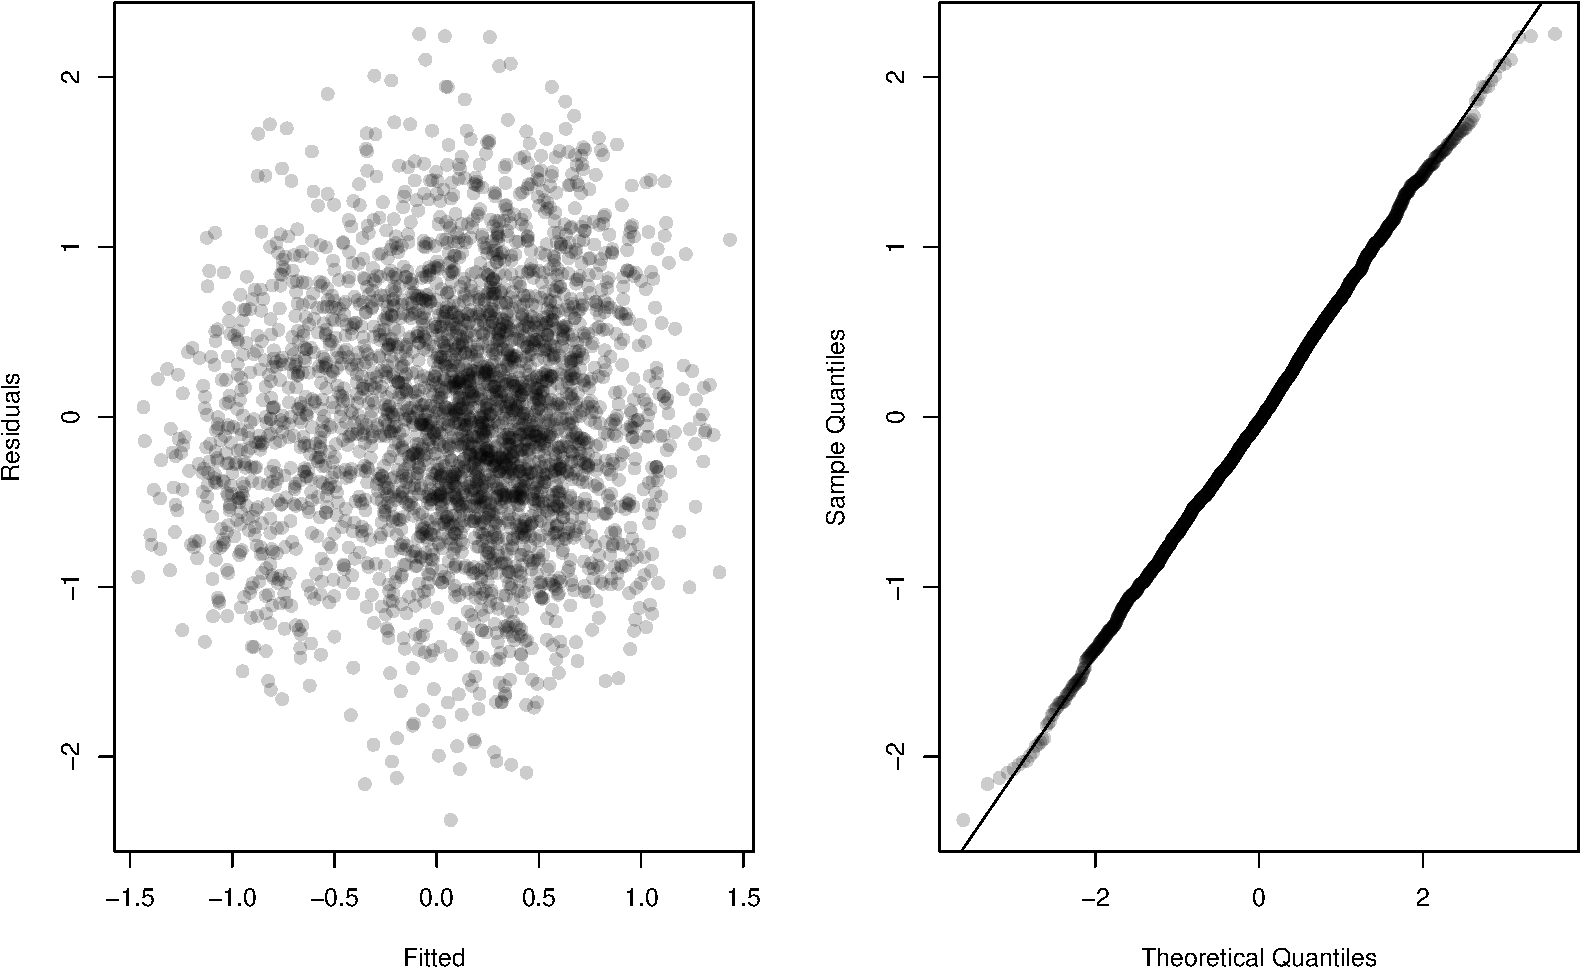
\includegraphics{week11p1_files/figure-beamer/unnamed-chunk-14-1.pdf}
\end{frame}

\begin{frame}{}
\protect\hypertarget{section-18}{}
We now investigate which genotypes are associated with AqE values that
are different than the RC reference level.

To do this we will consider a simple approach in which we construct a
model with a particular genotype level removed, and then compare this
smaller model with the final model.

Model comparisons will be made using AIC (the difference of AIC values).
We will perform this procedure for each genotype.

Results are displayed on later slides. Negative values indicate that a
genotype is associated with AqE values that are different than the RC
reference level.
\end{frame}

\begin{frame}[fragile]{}
\protect\hypertarget{section-19}{}
\small

\begin{Shaded}
\begin{Highlighting}[]
\DocumentationTok{\#\# AIC for each ID variable from full AqE fixed{-}effects model}
\NormalTok{M }\OtherTok{\textless{}{-}} \FunctionTok{model.matrix}\NormalTok{(AqE }\SpecialCharTok{\textasciitilde{}}\NormalTok{ ID }\SpecialCharTok{+}\NormalTok{ days }\SpecialCharTok{+} \FunctionTok{I}\NormalTok{(days}\SpecialCharTok{\^{}}\DecValTok{2}\NormalTok{) }\SpecialCharTok{+}\NormalTok{ Precip }\SpecialCharTok{+} 
\NormalTok{                    Precip\_7day, }\AttributeTok{data =}\NormalTok{ dat)}

\CommentTok{\# Note that likelihood ratios are asymptotic, i.e. don\textquotesingle{}t }
\CommentTok{\# account for uncertainty in the estimate of the residual }
\CommentTok{\# variance}
\FunctionTok{library}\NormalTok{(parallel)}
\NormalTok{ncores }\OtherTok{\textless{}{-}} \FunctionTok{detectCores}\NormalTok{() }\SpecialCharTok{{-}} \DecValTok{2}
\FunctionTok{system.time}\NormalTok{(\{AIC\_IDs }\OtherTok{\textless{}{-}} \FunctionTok{matrix}\NormalTok{(}\FunctionTok{unlist}\NormalTok{(}\FunctionTok{lapply}\NormalTok{(}
    \FunctionTok{grep}\NormalTok{(}\StringTok{"ID"}\NormalTok{, }\FunctionTok{colnames}\NormalTok{(M)), }\ControlFlowTok{function}\NormalTok{(j)\{}
\NormalTok{    M1 }\OtherTok{\textless{}{-}}\NormalTok{ M[, }\SpecialCharTok{{-}}\NormalTok{j]   }
\NormalTok{    foo }\OtherTok{\textless{}{-}} \FunctionTok{lmer}\NormalTok{(AqE }\SpecialCharTok{\textasciitilde{}} \SpecialCharTok{{-}}\DecValTok{1} \SpecialCharTok{+}\NormalTok{ M1 }\SpecialCharTok{+}\NormalTok{ (}\DecValTok{1}\SpecialCharTok{|}\NormalTok{plot\_number) }\SpecialCharTok{+}\NormalTok{ (}\DecValTok{1}\SpecialCharTok{|}\NormalTok{disk), }
                            \AttributeTok{data =}\NormalTok{ dat, }\AttributeTok{REML =} \ConstantTok{FALSE}\NormalTok{)}
    \FunctionTok{AIC}\NormalTok{(m\_re\_full) }\SpecialCharTok{{-}} \FunctionTok{AIC}\NormalTok{(foo) }
\NormalTok{\})), }\AttributeTok{ncol =} \DecValTok{1}\NormalTok{)\})}
\end{Highlighting}
\end{Shaded}

\begin{verbatim}
##    user  system elapsed 
##   4.470   0.095   4.566
\end{verbatim}
\end{frame}

\begin{frame}[fragile]{}
\protect\hypertarget{section-20}{}
\tiny

\begin{Shaded}
\begin{Highlighting}[]
\FunctionTok{rownames}\NormalTok{(AIC\_IDs) }\OtherTok{\textless{}{-}} \FunctionTok{colnames}\NormalTok{(M)[}\FunctionTok{grep}\NormalTok{(}\StringTok{"ID"}\NormalTok{, }\FunctionTok{colnames}\NormalTok{(M))]}
\FunctionTok{colnames}\NormalTok{(AIC\_IDs) }\OtherTok{\textless{}{-}} \FunctionTok{c}\NormalTok{(}\StringTok{"AqE"}\NormalTok{)}
\NormalTok{AIC\_IDs[AIC\_IDs }\SpecialCharTok{\textless{}} \DecValTok{0}\NormalTok{, ]}
\end{Highlighting}
\end{Shaded}

\begin{verbatim}
##        ID1        ID2        ID3        ID4        ID7        ID9       ID11 
## -2.9151635 -0.3967087 -0.8910848 -3.0220489 -5.7221648 -1.8426071 -1.1914115 
##       ID12       ID13       ID15       ID16       ID17       ID19       ID24 
## -0.6273336 -6.3892507 -4.5287970 -0.3193861 -8.2713125 -1.1833585 -7.6020182 
##       ID26       ID27       ID30       ID31       ID32       ID37       ID38 
## -5.9966713 -1.0398143 -1.4059465 -0.3284319 -2.4089731 -1.0959652 -3.6448254 
##       ID40 
## -4.8324469
\end{verbatim}
\end{frame}

\end{document}
